\documentclass[12pt, openany]{report}
\usepackage[utf8]{inputenc}
\usepackage[T1]{fontenc}
\usepackage{amsmath,amsfonts,amssymb}
\usepackage{amssymb}
\usepackage{multicol}
\usepackage[a4paper,left=2.5cm,right=2.5cm,top=2.5cm,bottom=2.5cm]{geometry}
\usepackage[english]{babel}
\usepackage{libertine}
\usepackage{graphicx}
\usepackage{wrapfig}
\usepackage{algorithm}
\usepackage{algpseudocode}
\usepackage{float}
\usepackage{enumitem}
\usepackage{pythonhighlight}
\usepackage[]{titletoc}
\usepackage{empheq}
\usepackage{titlesec}
\usepackage{mathpazo}
\usepackage{xfrac}
\usepackage{textcomp}
\usepackage{mathtools}
\usepackage{caption}
\usepackage{tabularray}
\usepackage{subcaption}
\usepackage[bottom]{footmisc}
\usepackage{pdfpages}
\usepackage{tabularx}
\usepackage{amsthm}
\usepackage[skins]{tcolorbox}
\titleformat{\chapter}[display]
  {\normalfont\bfseries}{}{0pt}{\Huge}
\usepackage{hyperref}
\newcommand{\hsp}{\hspace{20pt}}
\newcommand{\HRule}{\rule{\linewidth}{0.5mm}}
\newcommand{\R}{\mathbb{R}}
\newcommand{\C}{\mathbb{C}}
\theoremstyle{definition}
\newtheorem{thm}{Theorem}[chapter]
\newtheorem{definition}[thm]{Definition}
\newtheorem{lem}[thm]{Lemma}

\hbadness=100000
\begin{document}
\begin{titlepage}
    \begin{sffamily}
    \begin{center}
        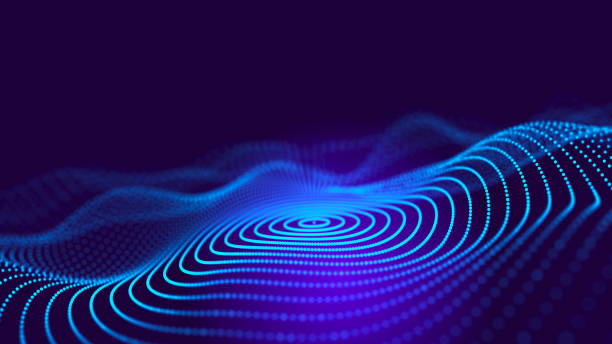
\includegraphics[scale=2.5]{img/page_de_garde.png} \\[1cm]
        \HRule \\[0.4cm]
        { \huge \bfseries LMECA2300 Advanced Numerical Methods \\[0.4cm] }
    
        \HRule \\[1.5cm]
        \textsc{\LARGE Simon Desmidt}\\[1cm]
        \vfill
        \vspace{2cm}
        {\large Academic year 2024-2025 - Q2}
        \vspace{0.4cm}
         
        
\includegraphics[width=0.15\textwidth]{img/epl.png}
        
        UCLouvain\\
    
    \end{center}
    \end{sffamily}
\end{titlepage}

\setcounter{tocdepth}{1}
\tableofcontents
\chapter{Definition of the problem}
\section{PDE}
The PDE that modelizes the behaviour of a 2D acoustic (or electromagnetic wave) is the following:
\begin{equation}
  	\rho_0 \frac{\partial \vec u}{\partial t}+\nabla p = r_v
\end{equation}
where $\rho_0$ is the average density of the environment, $\vec u$ the velocity of the wave, $p$ the variation of pressure and $r_v$ the pressure source. By the conservation laws, we can express it depending only on the pressure:
\begin{equation}
	\nabla^2 p - \rho_0 \chi \frac{\partial^2 p}{\partial t^2} = -\rho_0 \frac{\partial s_v}{\partial t}
\end{equation}
And we can express the speed as $v=1/\sqrt{\rho_0 \chi}$ whereas the impedance is $\eta = \sqrt{\frac{\rho_0}{\chi}}$. The plane wave is thus 
\begin{equation}
	p(x,t) = P_0 \cos (\omega t-kx)
\end{equation}
\section{Phasors}
Expressing the pressure as a phasor is much more easy to handle in the next parts. It is written as 
\begin{equation}
	p(\vec r,t) = Re\{P(\vec r)e^{j\omega_0 t}\}
\end{equation}
Furthermore, as we can express a plane wave as a cosine, 
\begin{equation}
	\cos(\omega t-kx) = Re(e^{j\omega t}e^{-jkx})
\end{equation}
And the relation with the Fourier transform is 
\begin{equation}
	\mathcal{F}(p) = P_r \pi[\delta (\omega-\omega_0) + \delta (\omega+\omega_0)] + jP_i \pi [\delta(\omega-\omega_0) - \delta(\omega+\omega_0)]
\end{equation}
\begin{figure}[H]
	\centering 
	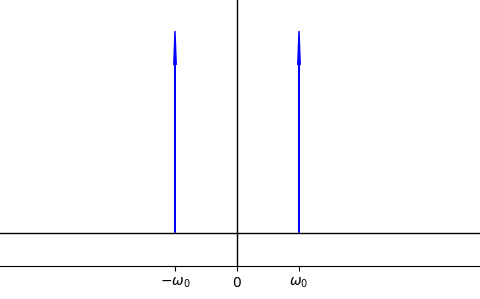
\includegraphics[width = .5\textwidth]{img/phasor.png}
\end{figure}
Using the phasor of the pressure, the wave equation becomes 
\begin{equation}
	\nabla^2 P + k^2 P = -j\omega_0 S_V
\end{equation}
\chapter{Basic resolution of the problem}
\section{Green's function}
Let us use a punctual term source $-\delta(x) \delta(y)$. The wave equation becomes
\begin{equation}
	\nabla^2 G + k^ G = -\delta(x)\delta(y)
\end{equation}
The solution is the Green function, that can be expressed as a linear combination of the Bessel functions of order 0:
\begin{equation}
	G(\rho) = AJ_0(k\rho) + BY_0(k\rho)
\end{equation}
where $\rho$ is the distance to the origin. 
\begin{figure}[H]
	\centering 
	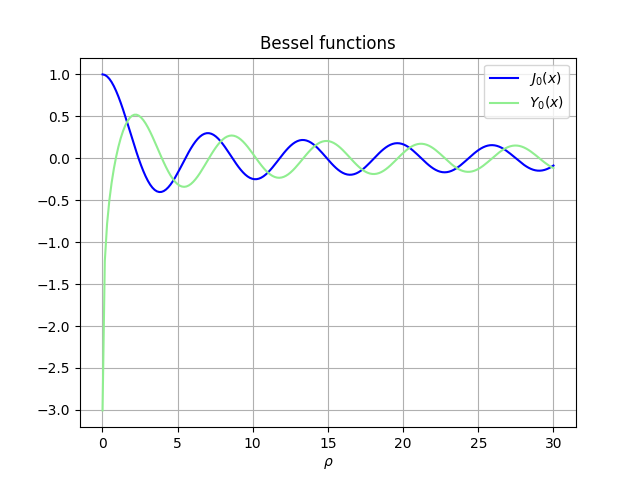
\includegraphics[width=.5\textwidth]{img/bessel.png}
\end{figure}
In our specific case, the solution is the Hankel function:
\begin{equation}
	G = -\frac{j}{4}H_0^{(2)}(k\rho) \qquad H_0^{(2)}(x) = J_0(x)-jY_0(x)
\end{equation}
And this can be approximated far from the origin:
\begin{equation}
	H_0^{(2)}(x) \approx \sqrt{\frac{2}{\pi x}} e^{j\pi/4} e^{-jx}
\end{equation}
\section{Radiation integral}
\subsection{One segment}
Gathering all these equations, the expression of the pressure due to a infinitesimal segment source $\Gamma'$ is 
\begin{equation}
	p(r) = G(\vec r-\vec r') (j\omega \rho_0) v_n(\vec r')d\Gamma '
\end{equation}
where $\vec r$ is the position of the observer, $\vec r'$ the position of the source and $v_n$ the normal velocity. \\
For a larger segment, the pressure is 
\begin{equation}
	p = p_{inc} + \frac{\omega \rho_0}{4}  \int_\Gamma H_0^{(2)}(k|\vec r-\vec r'|)v_n(\vec r') d\Gamma'
\end{equation}
This is the formula obtained from the convolution of the velocity source with the Green function. 
\subsection{Several segments}\label{sec:sev_seg}
If the object is made of several segments, we need to determine the importance of each of them in the radiation, to express the normal velocity:
\begin{equation}
	v_n = \sum_{i=1}^N x_i v_{n,i}
\end{equation}
In order to do that, we make the hypothesis that the pressure field is null in the middle of each segment, and we have a linear system to solve:
\begin{equation}
	p = 0 = \underbrace{p_ {inc}(\vec r_{mid, j})}_{\eqqcolon -b_j} + \sum_{i=1}^N x_i \frac{\omega \rho_0}{4} \underbrace{\int_{\Gamma'_i}  H_0^{(2)} (k|\vec r_{0,j}-\vec r'_i|) v_{n,i}(\vec r'_i) d\Gamma'_i}_{\eqqcolon A_{ij}}
\end{equation}
\begin{itemize}
	\item [$\to$] Note: the basis functions $v_{n,i}$ are nonzero on segment $i$ and null everywhere else. The nonzero value has no importance and can thus be 1 for all segments. 
\end{itemize}
The values of $b_j$ are computed using $p(\vec r) = P_0 e^{-jk \hat u\cdot \vec r}$. \\
The problem with this equation is that the Hankel function has a singularity at the origin, but is still integrable. This means that we have to find a trick to integrate it numerically. \\
Around the origin, we have the approximation
\begin{equation}
	H_0^{(2)}(x) \approx 1-j\frac{2}{\pi}(\ln(x/2)+\gamma)
\end{equation}
with $\gamma$ the Euler constant. We can use that on the following expression, to get rid of the singular behaviour in the integration: 
\begin{equation}
	H_0^{(2)}(x) = \left(H_0^{(2)}(x) + j\frac{2}{\pi}\ln(x)\right) - j\frac{2}{\pi} \ln(x)
\end{equation}
where the integration of the last $\ln$ is done analytically. 
\chapter{Multipole Method}
\section{Definition of the method}
The basic idea of the multipole method in the context of the acoustic waves is to decompose a circular wave into an infinite number of planar wave. The goal is to accelerate the integration process by computing some terms one single time for a lot of points. 
\begin{figure}[H]
	\centering 
	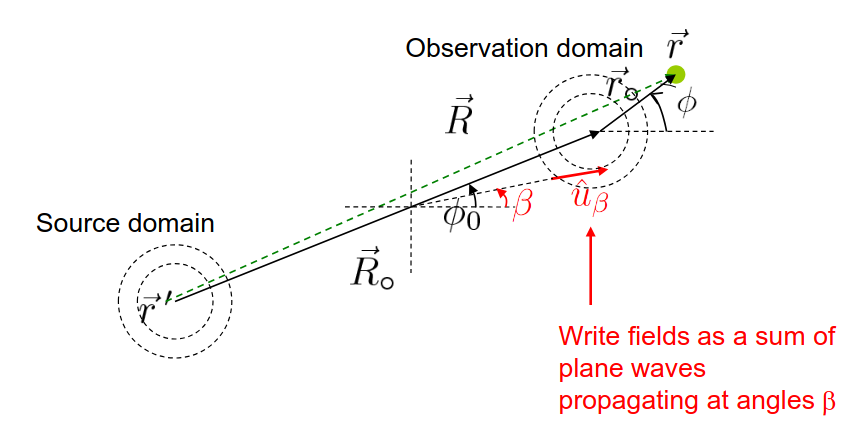
\includegraphics[width=.6\textwidth]{img/multipole.png}
\end{figure}
To achieve this goal, we take a reference point of the sources $\vec r'$ (noted $A$) and a reference point for the observation domain $\vec r_0$ (noted $B$). \\
To get the final results, we use different formulas:
\begin{itemize}
	\item Superposition of waves: $H_0^{(2)}(kR) = \sum_{l=0}^\infty H_l^{(2)}(kR_0)\cos(l(\phi-\phi_0)) \epsilon(l)J_l(kr_0)$, where $\epsilon(l) = 1$ if $l=0$ and $2$ otherwise; 
	\item Anger-Jacobi: $\cos(l(\phi-\phi_0)) J_l(kr_0) = \frac{1}{2\pi} (-j)^l \int_0^{2\pi} \cos(l(\beta-\phi_0)) e^{-jk\hat u_\beta \cdot \vec r_0} d\beta$, where $\beta$ is the incident angle of the planar waves;
\end{itemize}
This approximation is correct only in a relatively small zone around the point $B$, and far from the source. This means that for a large domain, we can take several boxes around points $B_k$, and compute for each smaller domain using the multipole method. This is the aim of this course. Note that in the close field around the source object, we have to continue using the method seen previously. 
\section{Final formula}
The final integration formula for our radiation problem is the following:
\begin{equation}
	p = \sum_{i=0}^N \int_{S'} H_0^{(2)} (k|\vec r-\vec r'|)v_i(\vec r')dS' \approx \frac{1}{2\pi} \int_0^{2\pi} e^{-jk\hat u_\beta \cdot \vec r_0} \sum_{i=1}^N x_i F_i(\beta) T(k,\beta,R_0)d\beta 
\end{equation}
where 
\begin{itemize}
	\item $F_i(\beta) = \int_{S'_i} v_{n,i}(\vec r') e^{jk \hat u_\beta \cdot \vec r_0'}dS'_i = e^{jk \hat u_\beta \cdot (\vec r_1- A)} \| \vec r_2-\vec r_1\| \frac{\sin(p)}{p} e^{jp}$ with $p=k\hat u_\beta \cdot (\vec r_2-\vec r_1)/2$; 
	\item $T(k, R_0, \beta) = \sum_{l=0}^L c(l) \cos(l(\beta-\phi_0)) H_l^{(2)}(kR_0)$ with $c(l) = \epsilon(l)(-j)^l$;
\end{itemize}
The whole point of this method is that most of the computation can be done before calculating the pressure field: the $F_i(\beta)$ coefficients can be calculated once for the whole problem as it depends only on the number of planar waves we are using. The terms $T(k,R_0,\beta)$ needs to be calculated once for each $\beta$ in each box. It is however a small number of computations if the boxes are chosen correctly. The final term is the exponential, which has to be computed for each point of the domain, but does not take much time as it only contains a 2D dot product. The easiest way to get rid of the integral is by using a Riemann sum to approximate it. 
\begin{itemize}
	\item [$\to$] Note: the only method to compute the coefficients $x_i$ is through the linear system of section \ref{sec:sev_seg}.
\end{itemize} 
\end{document}